\documentclass{beamer}

\usepackage[frenchb]{babel}
\usepackage[T1]{fontenc}
\usepackage[utf8]{inputenc}

\usetheme{Warsaw}

\title{IDS - Suricata / Snort}
\author{Aurélien Monnet-Paquet}
\institute{www.inria.fr}
\date{17 Mars 2016}

\begin{document}

%Premiere page : page de garde.
\begin{frame}
\titlepage
\end{frame}

%Deuxieme page : Qu'est ce qu'un IDS ?
\section{Présentation}
\subsection{Les IDS}
\begin{frame}
\frametitle{Qu'est ce qu'un IDS ?}
\begin{itemize}
\setbeamertemplate{itemize item}[triangle]
\item Systèmes de détection d'intrusion
\item Écoute le réseau de manière furtive afin de repérer des activités suspectes
\pause
\item Placement de l'IDS au niveau du routeur de sortie/d'entrée du réseau
\pause
\item Et la concurrence ? Snort Suricata Bro ...
\end{itemize}
\end{frame}

%Troisieme page : But de suricata
\subsection{Suricata}
\begin{frame}
\frametitle{But de Suricata (2008)}
\begin{itemize}
\setbeamertemplate{itemize item}[triangle]
\item Apporter de nouvelles technologies aux IDS :
\begin{itemize}
\item Performance : Le multi-threads
\item Accélération matérielle (par GPU)
\end{itemize}
\item Support d'IPv6 natif
\item Open source
\item Disponible sur Linux / MAC / Windows
\item Supporte presque toutes les signatures de snort
\end{itemize}
\end{frame}

%4 eme page : Les projets similaires
\subsection{Les projets similaires}
\begin{frame}
\frametitle{Snort et Bro}
\begin{itemize}
\setbeamertemplate{itemize item}[triangle]
\item Snort
\begin{itemize}
\item Développé par Sourcefire
\item Fonctionnellement équivalent à Suricata
\item Compatibilité Snort / Suricata
\item Concurrence directe
\end{itemize}
\pause
\item Bro
\begin{itemize}
\item Orientation capture
\item Études statistiques
\end{itemize}
\end{itemize}
\end{frame}

%Partie II : Fonctionnement
%5 eme page : Fonctionnement en interne.
\section{Fonctionnement}
\subsection{En interne}
\begin{frame}
\frametitle{Fonctionnement}
\begin{itemize}
\setbeamertemplate{itemize item}[triangle]
\item Lève une alerte mais ne bloque pas le flux (rôle de l'IPS)
\item Travail avec un flux de données
\item Reconstruction du flux : TCP => perte/renvoi/ordre
\item La réception d'un ACK déclenche l'analyse des données.
\end{itemize}
\begin{center}
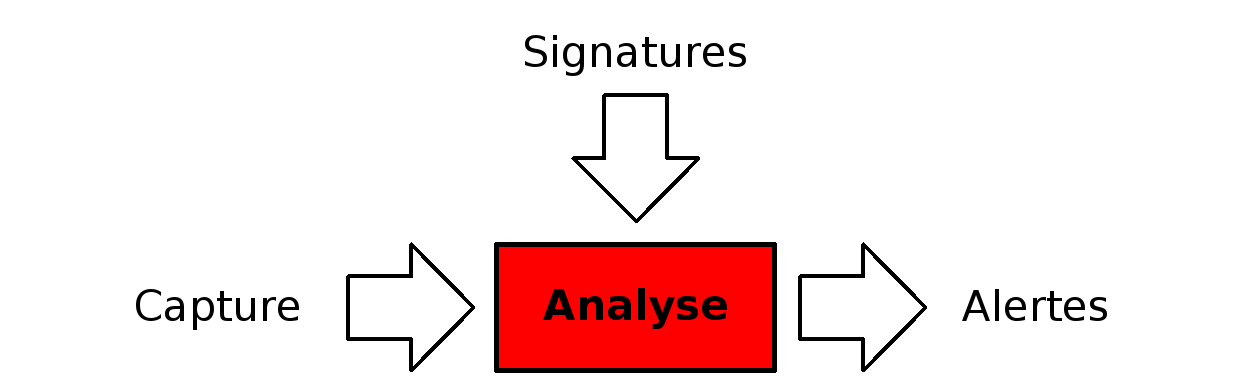
\includegraphics[scale=0.15]{img/matching.png}
\end{center}
\end{frame}

%6 eme page : Exemple de regles (Actions)
\subsection{Exemple de règles}
\begin{frame}
\frametitle{Fonctionnement des règles de matching}
\begin{center}
\textcolor{red}{alert} http any any $\rightarrow$ any any (msg:""; content:"inria.fr";)
\end{center}
Actions :
\begin{enumerate}
\item pass
\item drop
\item reject
\item alert
\end{enumerate}
\end{frame}

%7 eme page : Exemple de regles (http)
\begin{frame}
\frametitle{Fonctionnement des règles de matching}
\begin{center}
alert \textcolor{green}{http} any any $\rightarrow$ any any (msg:""; content:"inria.fr";)
\end{center}
Protocole :
\begin{itemize}
\setbeamertemplate{itemize item}[triangle]
\item tcp / udp
\item ip
\item icmp
\end{itemize}
\end{frame}

%8 eme page : Exemple de regles (Source / Destination)
\begin{frame}
\frametitle{Fonctionnement des règles de matching}
\begin{center}
alert http \textcolor{blue}{any any}  $\rightarrow$ \textcolor{blue}{any any} (msg:""; content:"inria.fr";)
\end{center}
Source/Destination Port :
\begin{itemize}
\setbeamertemplate{itemize item}[triangle]
\item 128.93.162.84 80 $\rightarrow$ 192.168.17.218 any
\item $\$EXTERNAL\_NET$ any <> $\$HOME\_NET$ any
\end{itemize}
\end{frame}

%9 eme page : Exemple de regles (Motif)
\begin{frame}
\frametitle{Fonctionnement des règles de matching}
\begin{center}
alert http any any $\rightarrow$ any any (msg:""; \textcolor{cyan}{content:"inria.fr";})
\end{center}
\begin{center}
Motif
\end{center}
\end{frame}

%10 eme page : Exemple de regles (autre parametres)
\begin{frame}
\frametitle{Fonctionnement des règles de matching}
\begin{center}
alert http any any $\rightarrow$ any any (\textcolor{cyan}{msg:"";} content:"inria.fr";)
\end{center}
Autres paramètres :
\begin{itemize}
\setbeamertemplate{itemize item}[triangle]
\item msg:"Connexion établie depuis le site www.inria.fr"
\item http\_uri, http\_method, http\_header, http\_cookie $\ldots$
\item flow:established,to\_server; to\_client; nocase; $\ldots$
\end{itemize}
\end{frame}

% Partie III
%11 eme page : Fonctionnalitée avancée.
\section{Fonctionnalité avancée}
\subsection{libhtp}
\begin{frame}
\frametitle{Suricata et LibHtp}
\begin{itemize}
\item Capable de décoder des flux compressé par Gzip.
\item flow:to\_client; content:"Inria recrute"; nocase; $ \Rightarrow $ Page web non compressé.
\end{itemize}
\end{frame}

\end{document}